\documentclass[11pt]{sdm}
\usepackage{graphicx}
\usepackage{subcaption}
\usepackage{textcomp}
\usepackage[francais]{babel}

%numeroter les pages
\pagestyle{plain}

\title{Deep Learning and Time Series}
\author{Arthur \textsc{Le Guennec}}
\supervisorOne{Romain \textsc{Tavenard} of your first supervisor}
\supervisorTwo{Simon \textsc{Malinowski} of your second supervisor}
\team{OBELIX}
%One of:
% ens-Rennes  esir    insa-rennes logoENIB  rennes1  UBO
% enssat header logo_ENIB   logoUbs   tel-br supelec

\school{rennes1}


% the domain should be one or two of
% Technology for Human Learning 
% Artificial Intelligence				***** 
% Computer Arithmetic
% Hardware Architecture
% Automatic Control Engineering
% Bioinformatics 
% Biotechnology
% Computational Complexity 
% Computational Engineering, Finance, and Science
% Computational Geometry 
% Computation and Language 
% Cryptography and Security 
% Computer Vision and Pattern Recognition
% Computers and Society 
% Databases 							*****
% Distributed, Parallel, and Cluster Computing 
% Digital Libraries
% Discrete Mathematics 
% Data Structures and Algorithms 
% Embedded Systems 
% Emerging Technologies 
% Formal Languages and Automata Theory 
% General Literature 
% Graphics 
% Computer Science and Game Theory 
% Human-Computer Interaction 
% Computer Aided Engineering 
% Medical Imaging 
% Information Retrieval 
% Information Theory 
% Ubiquitous Computing 
% Machine Learning						*****
% Logic in Computer Science 
% Multiagent Systems 
% Mobile Computing
% Multimedia
% Modeling and Simulation 
% Mathematical Software 
% Numerical Analysis 
% Neural and Evolutionary Computing 
% Networking and Internet Architecture 
% Operating Systems 
% Performance 
% Programming Languages 
% Robotics 
% Operations Research
% Symbolic Computation 
% Sound
% Software Engineering 
% Social and Information Networks 
% Systems and Control 
% Image Processing 
% Signal and Image Processing 
% Document and Text Processing
% Web
\domain{Domain:  (examples) Data Structures and Algorithms - Logic in Computer Science}

%write your abstract here
\abstract{write your abstract here}



\begin{document}
\maketitle

%*****************************************************************%

\section{Introduction}

Beaucoup d\textquotesingle articles sur la classification des s\'eries temporelles ont \'et\'e \'ecrits, et est pr\'esente dans beaucoup de domaine comme la m\'edecine, la biologie, la reconnaissance audio, ... Il existe aussi beaucoup de m\'ethodes diff\'erentes pour y parvenir. Par exemple, l\textquotesingle article de Bailly et coll. (\cite{bailly2015bag}) utilise les bag-of-words, une technique bas\'ee sur la description des documents par des mots. \cite{zheng2014time} utilise plut\^ot les r\'eseaux de neurones convolutionnels.
Dans ce document, nous allons utiliser les r\'eseaux de neurones profonds. Dans ce type de mod\`ele d\textquotesingle apprentissage, les r\'eseaux convolutionnels (ou Convolutional Neural Networks) donnent de tr\`es bons r\'esultats dans le domaine de la classification d\textquotesingle image (\cite{chatfield2014return}).
Comme dans le domaine des s\'eries temporelles les nombres de donn\'ees annot\'ees est faible, et que les architectures qui vont seront utilis\'e demandent beaucoup de donn\'ee afin de fonctionner correctement. Nous allons donc explorer les m\'ethodes permettant de diminuer les cons\'equequences de ce manque de donn\'ees. \\
Ce papier est organis\'e de la mani\`ere suivante. La section 2 concerne l\textquotesingle \'etat de l\textquotesingle art dans ce domaine, et la section 3 s\textquotesingle interessera aux probl\`emes du manque de donn\'ees pour les s\'eries temporelles.

% Ce sujet de stage propose de s’int\'eresser \`a la classification de s\'eries temporelles en utilisant des mod\`eles d\textquotesingle apprentissage tr\`es puissants : les r\'eseaux de neurones profonds (Deep Neural Networks). Dans cette famille de m\'ethodes, les r\'eseaux convolutionnels (Convolutional Neural Networks, CNN) montrent actuellement l\textquotesingle \'etendue de leurs capacit\'es dans le domaine de la vision par ordinateur (voir par exemple [1]). Les tr\`es bonnes performances des CNN s’expliquent par leur capacit\'e \`a tirer profit des grands volumes de donn\'ees disponibles pour apprendre des descriptions et des classifieurs complexes. Dans le domaine de la classification de s\'eries temporelles, les volumes de donn\'ees annot\'ees sont souvent bien plus faibles [2]. l\textquotesingle objet de ce stage est d\textquotesingle \'evaluer la pertinence de l\textquotesingle utilisation des CNN dans ce cadre et de proposer des moyens d\textquotesingle att\'enuer l\textquotesingle impact attendu du faible volume de donn\'ees annot\'ees [3]. l\textquotesingle \'etudiant(e) retenu(e) devra faire preuve d\textquotesingle organisation et de s\'erieux pour mener \`a bien la campagne exp\'erimentale intensive impliqu\'ee par ce sujet. Pour ce faire, il/elle utilisera le framework Caffe [4].
 

\section{\'Etat de l\textquotesingle art}
	La classification de s\'erie temporelle est un sujet qui est \'etudi\'e depuis maintenant plusieurs ann\'ees, et diff\'erentes techniques existent et de nombreux articles ont \'et\'e \'ecrits sur le sujet. Dans cette partie nous allons voir quelques unes de ces diff\'erentes techniques.

	\subsection{Ce qui ce fait actuellement}
		\subsubsection{D\'eformation dynamique temporelle}
			La d\'eformation dynamique temporelle (ou DTW en anglais pour Dynamic Time Warping) est un algorithme qui permet de detecter si deux s\'eries ont des similarit\'e m\^eme s\textquotesingle il y a eu une d\'eformation (figure~\ref{fig:dtw}).

			\begin{figure}[!ht]
				\centering
				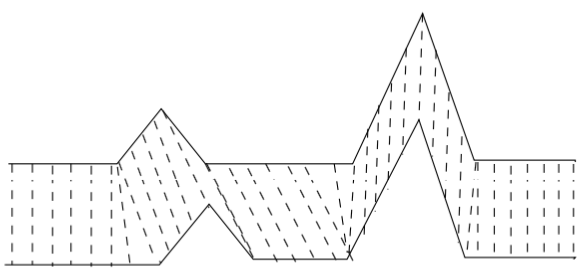
\includegraphics[scale=0.6,natwidth=582,natheight=269]{figures/dtw.png}
				\caption{Exemple de deux s\'eries temporelles diff\'erentes mais avec un sch\'ema similaire.}
				\label{fig:dtw}
			\end{figure}

		\subsubsection{Bag-of-Words}	
			Le Bag-of-Words (BoW) est un mod\`ele de description de document avec des descripteurs (qui sont consid\'er'es comme des mots). Il fonctionne en attribuant des mots aux documents, chaque mot ayant un probabilit\'e par par document (figure~\ref{fig:BoW}). L\textquotesingle article de Bailly et coll. \cite{bailly2015bag} traite justement le sujet de la classification des s\'eries temporelles avec les Bag-of-Words. En utilisant les maximums et minimums locaux, ils obtiennent des mots qui seront ensuite utilis\'es dans la description des s\'eries temporelles.

			\begin{figure}[!ht]
				\centering
				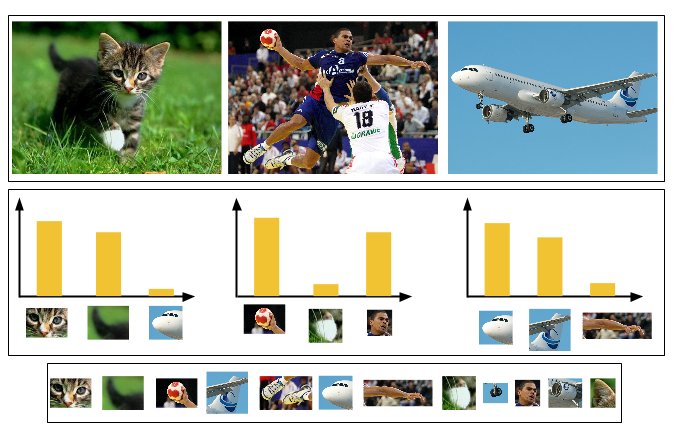
\includegraphics[scale=0.6,natwidth=680,natheight=440]{figures/bagOfWords.png}
				\caption{Le bag-of-words est en bas de la figure, il est compos\'e de diff\'erents mots, ici des images, qui sont reconnus sur les documents (en haut), qui sont ici des images. Par exemple, pour la premi\`ere image, on a une forte correspondance avec le premier et deuxi\`eme mot, alors que l\textquotesingle on a une faible correspondance avec la derni\`ere image.}
				\label{fig:BoW}
			\end{figure}

			En utilisant l\textquotesingle algorithme de SIFT (Scale-Invariant Feature Transform) sur les donn\'ees d\textquotesingle UCR (\cite{UCRArchive}), les taux d\textquotesingle erreurs obtenus dans \cite{bailly2015bag} sont parfois meilleurs qu'en utilisant le DTW (Dynamic Time Warping) et la m\'ethode des k plus proches voisins seuls.

	\subsection{R\'eseau de neurones}
		Les r\'eseaux de neurones sont un syst\`eme inspir\'e du mod\`ele biologique du cerveau. Un r\'eseau de neurone est compos\'e de plusieurs neurones (figure~\ref{fig:neuralNetwork}) qui ont chacun une fonction d\textquotesingle activation (figure~\ref{fig:neural}) et qui sont reli\'es \`a d\textquotesingle autres neurones par des poids.
		La taille de la base de donn\'ee utilis\'ee influence aussi les r\'esultats, Par exemple, l'article de ??? [J\textquotesingle ai oubli\'e la r\'ef\'erence] montre que les performances d\'ependent de la taille des donn\'ees utilis\'ees.

		\subsubsection{Un r\'eseau de neurone en g\'en\'eral}
			\begin{itshape}Les neurones\end{itshape}
			\smallbreak
			Un neurone est une unit\'e qui contient une fonction d\textquotesingle activation qui d\'efini son comportement. La figure~\ref{fig:neural} repr\'esente un neurone qui a 4 entr\'ees et une sortie. On note \texbf{$X$} le vecteur d\textquotesingle entr\'ee, \textbf{$W$} le vecteur des poids, $b$ le biais, $f(.)$ la fonction d\textquotesingle activation, et $h(X)$ la sortie du neurone. Notons aussi $z$ la somme des poids et $n$ le nombre d\textquotesingle entr\'ee d\textquotesingle un neurone (sans compter le biais). On a donc les \'equations suivantes :
			
			\begin{equation}
				z = \sum_{k=0}^n w_k x_k + b
				\label{eq:z}
			\end{equation}

			\begin{equation}
				h_{W,b}(X) = f(z)
				\label{eq:h}
			\end{equation}

			\begin{figure}[!ht]
				\centering
				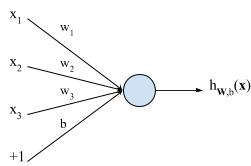
\includegraphics[scale=0.7,natwidth=251,natheight=166]{figures/neural.png}
				\caption{Comme on peut le voir, le neurone ci-dessus re\c coit 4 valeurs, dont le biais. Dans un r\'eseau de neurones, les entr\'ees $x$ sont en faite les sorties d\textquotesingle autres neurones.}
				\label{fig:neural}
			\end{figure}

			Un neurone seul ne peut pas effectuer de t\^ache, c\textquotesingle est pourquoi ils sont utilis\'es \`a plusieurs pour effectuer diverses t\^aches comme de l\textquotesingle analyse de donn\'ee ou de la classification.	

			\medbreak
			\begin{itshape}L\textquotesingle architecture\end{itshape}
			\smallbreak
			L\textquotesingle efficacit\'e d\textquotesingle un r\'eseau de neurones d\'epend de son architecture.
			Il existe diff\'erentes architectures pour un r\'eseau de neurone (figure~\ref{fig:neuralNetwork}), la plus connue et la plus r\'epandue \'etant le r\'eseau de neurone non-boucl\'e (ou feedfoward neural network en anglais) (figure~\ref{fig:nnl}). Selon le nombre de couche cach\'ee et le nombre de neurones par couche, le r\'eseau peut \^etre plus ou moins performants (\cite{chatfield2014return}, \cite{srivastava2014dropout}). 

			\begin{figure}[!ht]
				\centering
				\begin{subfigure}{0.45\textwidth}
					\centering	
					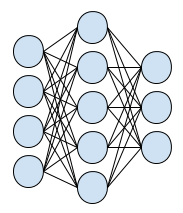
\includegraphics[scale=0.7,natwidth=183,natheight=213]{figures/neuralNetworkLayers.png}
					\caption{R\'eseau de neurones \`a couches}
					\label{fig:nnl}
				\end{subfigure}
				\hspace*{\fill}
				\begin{subfigure}{0.45\textwidth}	
					\centering
					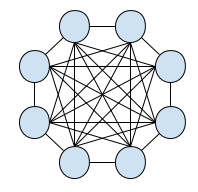
\includegraphics[scale=0.7,natwidth=198,natheight=192]{figures/neuralNetworkCompleteConnexion.png}
					\caption{R\'eseau de neurones \`a connexion compl\`ete}
					\label{fig:nnc}
				\end{subfigure}
				\caption{Il existe diff\'erents types de r\'eseaux de neurones. Par exemple, la figure 1.a est un r\'eseau avec une architecture \`a couche, alors que le r\'eseau de la figure 2.b \`a une architecture \`a connexion compl\`ete. Dans le domaine de la classification, l\textquotesingle architecture \`a couche est souvent utilis\'e.}
				\label{fig:neuralNetwork}
			\end{figure}
			
			Pour faire fonctionner un r\'eseau de neurone non-boucl\'e, on lui transmet une entr\'ee qui est de la m\^eme taille que la couche d\textquotesingle entr\'ee (par exemple, si l\textquotesingle entr\'ee est une image, sa taille peut correspondre au nombre de pixel). Ces valeurs sont ensuite transmises aux neurones de la couche suivante de mani\`ere repet\'ee jusqu\textquotesingle \`a couche de sortie.

			En appliquant les formules \ref{eq:z} et \ref{eq:h}, et en notant $L$ le nombre de couche dans le r\'eseau, $a$ l\textquotesingle activation d\textquotesingle un neurone (qui correspond \`a la sortie du neurone), $n^{(l)}$ le nombre de neurone de la couche $l$, $w_{ij}^{(l)}$ le poids allant du neurone $j$ de la couche $l-1$ au neurone $i$ de la couche $l$, $x$ le vecteur d\textquotesingle entr\'ee du r\'eseau, on obtient les \'equations suivantes :

			\begin{equation}
				a_i^{(0)} = x_i
				\label{eq:input}
			\end{equation}

			\begin{equation}
				z_i^{(l)} = \sum_{k=0}^{n^{(l-1)}} w_{ik}^{(l)} a_k^{(l-1)} \enskip \forall 1 < l \leq L
				\label{eq:zGlobal}
			\end{equation}

			\begin{equation}
				a_i^{(l)} = f(z_i^{(l)}) \enskip \forall 1 < l \leq L
				\label{eq:activation}
			\end{equation}

			\medbreak
			\begin{itshape}L\textquotesingle apprentissage\end{itshape}
			\smallbreak
			Il existe diff\'erentes types d\textquotesingle apprentissage, les trois principaux \'etant l\textquotesingle apprentissage supervis\'e, l\textquotesingle apprentissage non-supervis\'e et l\textquotesingle apprentissage par renforcement.
			L\textquotesingle apprentissage supervis\'e consiste \`a forcer le r\'eseau \`a converger vers un \'etat souhait\'e et n\'ecessite donc des donn\'ees labell\'ees.
			L\textquotesingle apprentissage non-supervis\'e consiste \`a converger le r\'eseau vers n\'importe quel \'etat et ne necessite pas de donn\'ees non-labell\'ees
			L\textquotesingle apprentissage par renforcement consiste \`a apprendre au r\'eseau \`a s\textquotesingle adapter par rapport aux diff\'erentes situations. 
			
			Pour la classification de s\'eries temporelles, nous utiliserons l\textquotesingle apprentissage supervis\'e.
			C\textquotesingle est durant l\textquotesingle apprentissage que l\textquotesingle on trouve les poids qui lient les neurones. Le m\'ethode la plus souvent utilis\'ee est la backpropagation qui consiste \`a diminuer l\textquotesingle erreur de la sortie, l\textquotesingle erreur \'etant la diff\'erence entre la valeur obtenue et la valeur souhait\'ee dans le cas d\textquotesingle un apprentissage supervis\'e. Cette diff\'erence est aussi appel\'e la fonction de co\^ut et est not\'e $J(W,b;x,y)$ avec $W$ la matrice des poids, $b$ le vecteur des biais, $x$ le vecteur d\textquotesingle entr\'ee, et $y$ le vecteur de sortie esp\'er\'e. Le but est donc bien de diminuer au maximum cette fonction de co\^ut. Dans le tutoriel de Ng et coll. (\cite{ng2012ufldl}), cette fonction de co\^ut est d\'ecrite par l\textquotesingle equation suivante :

			\begin{equation}
				J(W,b;x,y) = \frac{1}{2} {\left\Vert h_{W,b}(x) - y \right\Vert}^2
				\label{eq:costFunction}
			\end{equation}

			Une fois cette fonction trouv\'ee, on applique une descente de gradient sur les param\^etres $W$ et $b$. On a donc :

			\begin{equation}
				W_{ij}^{(l)} = W_{ij}^{(l)} - \alpha \frac{\partial}{\partial W_{ij}^{(l)}} J(W,b)
				\label{eq:gradientDescentWeight}
			\end{equation}
 
			\begin{equation}
				b_{i}^{(l)} = b_{i}^{(l)} - \alpha \frac{\partial}{\partial b_{i}^{(l)}} J(W,b)
				\label{eq:gradientDescentBiaises}
			\end{equation}

			$\alpha$ correspond au taux d\textquotesingle apprentissage et doit \^etre soigneusement choisi. Si $\alpha$ est trop grand, on risque de louper les bonnes valeurs. Si $\alpha$ est trop petit, l\textquotesingle apprentissage sera plus long, mais on risque surtout de rester bloquer dans un extremum local. Pour r\'esumer les formules (\ref{eq:costFunction}), (\ref{eq:gradientDescentWeight}) et (\ref{eq:gradientDescentBiaises}), on part de la sortie du r\'eseau de neurone pour revenir jusqu\textquotesingle \`a l\textquotesingle entr\'ee tout en modifiant sur le chemin les poids qui relient les neurones entre chaque couche. On relance ensuite le r\'eseau de neurone avec la m\^eme donn\'ee.
			On recommence ce processus selon diverses conditions, comme un nombre fix\'e \`a l\textquotesingle avance, un taux d\textquotesingle erreur atteint, ...
			On relance tout ce processus autant de fois que l\textquotesingle on a de donn\'ees d\textquotesingle entra\^inement.

			\medbreak
			\begin{itshape}Le sur-appprentissage et le sous-apprentissage\end{itshape}
			\smallbreak
			L\textquotesingle apprentissage conna\^it deux probl\`emes principaux, le sur-apprentissage (overfitting en anglais) et le sous-apprentissage (underfitting en anglais).
			Le sur-apprentissage appara\^it lorsque le r\'eseau de neurone s\textquotesingle est trop sp\'ecialis\'e. Cela arrive lorsque l\textquotesingle on entra\^ine le r\'eseau sur le m\^eme jeu de donn\'ee trop de fois. Par exemple, la figure~\ref{fig:overfitting} montre un exemple de sur-apprentissage, la courbe rouge \'etant bien capable de de retrouver les donn\'ees d\textquotesingle entra\^inement, mais serait incapable de retrouver une donn\'ee se situant sur la courbe verte.

			Le sous-apprentissage est lui un probl\`eme de manque d\textquotesingle entra\^inement. Comme on peut le voir sur la figure~\ref{fig:underfitting}, la courbe rouge ne s\textquotesingle est pas assez sp\'ecialis\'ee contrairement au cas du sur-apprentissage.


			\begin{figure}[!ht]
				\centering
				\begin{subfigure}{0.45\textwidth}
					\centering
					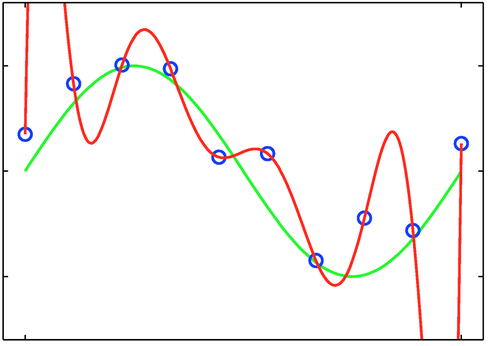
\includegraphics[natwidth=489,natheight=346,width=200,height=140]{figures/overfitting.png}
					\caption{Sur-apprentissage}
					\label{fig:overfitting}
				\end{subfigure}
				\hspace*{\fill}
				\begin{subfigure}{0.45\textwidth}	
					\centering
					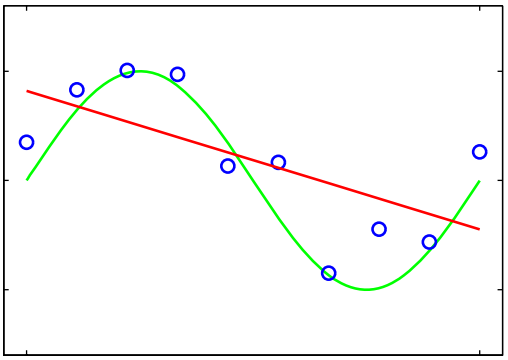
\includegraphics[natwidth=508,natheight=360,width=200,height=140]{figures/underfitting.png}
					\caption{Sous-apprentissage}
					\label{fig:underfitting}
				\end{subfigure}
				\caption{Les points bleus sont les donn\'ees \`a apprendre, la courbe verte est la fonction que l\textquotesingle on aimerait avoir, et la courbe rouge est la fonction que l\textquotesingle on a obtenu.}
			\end{figure}



			\medbreak

		\subsubsection{R\'eseau de neurones profond}
			Un r\'eseau de neurones profond est un r\'eseau qui contient plusieurs couches cach\'ees. Ce type de r\'eseau a l\textquotesingle avantage de pouvoir apprendre un plus grand nombre de fonction avec un nombre de neurone dans les couches cach\'ees bien inf\'erieurs \`a celui d\textquotesingle un r\'eseau classique. En effet, \`a la place d\textquotesingle avoir un nombre exponentielle de neurones cach\'es (par rapoort aux neurones d\textquotesingle entr\'es), nous avons un nombre polynomiale.
			Cependant, les r\'eseaux de neurones profonds sont difficiles \`a entra\^iner car ils n\'ecessitent beaucoup de donn\'ees label\'ees. L\textquotesingle entra\^inement d\textquotesingle un r\'eseau avec peu de donn\'ees nous donnerait un sur-apprentissage. De plus, l\textquotesingle entra\^inement par backpropagation vu \`a la section d\textquotesingle est peu efficace s\textquotesingle il est utlis\'e directement et induit souvent en erreur (du aux extremum locaux). Il faut donc les entra\^iner diff\'errement.
			Une des m\'ethodes existantes est greedy layerwise training qui consiste \`a d\textquotesingle abord entra\^iner un r\'eseau avec une couche cach\'ee, de garder les param\`tres obtenus, puis de rajouter une seconde couche cach\'ee, et ainsi de suite (figure~\ref{fig:trainDeepNet}).

			\begin{figure}[!ht]
				\centering
				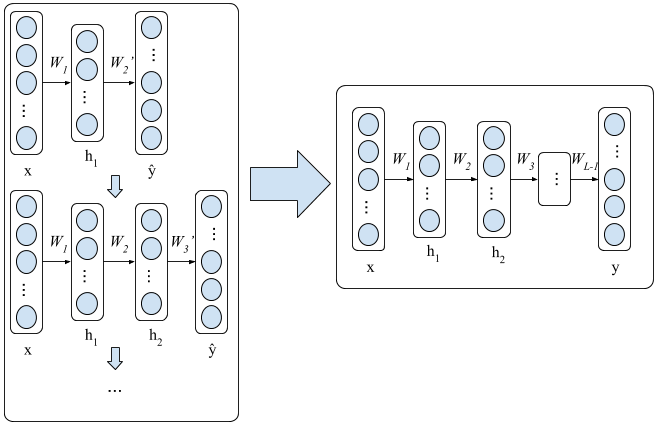
\includegraphics[scale=0.5,natwidth=919,natheight=412]{figures/trainDeepNetByGreedyLayerWise.png}
				\caption{On utilise ici l\textquotesingle algorithme greedy layerwise training avec des stacked autoencoders. C\textquotesingle est \`a dire que l\textquotesingle on veut que la sortie soit le plus proche possible de la couche qui la prec\`ede.}
				\label{fig:trainDeepNet}
			\end{figure}

		\subsubsection{R\'eseau de neurones convolutionnels}
			Les CNN (Convolutional Neural Network, ou r\'eseaux convolutionnels) sont un structure particuli\`ere des r\'eseaux de neurones profond car les neurones d\textquotesingle une couche \`a une autre ne sont pas tous reli\'es entre eux. En effet, es connections entre neurones se font localement, ce qui fait des entr\'ees d\textquotesingle une couche cach\'ee un sous-ensemble de motif de la couche pr\'ec\'edente (figure~\ref{fig:cnn}.

			\begin{figure}[!ht]
				\centering
				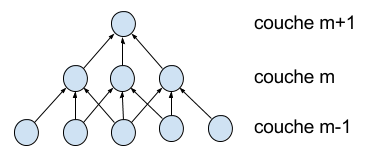
\includegraphics[natwidth=375,natheight=152]{figures/architectureCNN.png}
				\caption{Ici, imaginons que la couche m-1 est une r\'etine o\`u chaque neurone correspond \`a un pixel d\textquotesingle une image. Dans la couche m, on s\textquotesingle aper\c coit que chaque neurone a 3 entr\'ees qui correspondent chacune \`a un pixel. Chaque neurone de la couche m est donc un sous-ensemble de l\textquotesingle image de 3 pixels. De la m\^eme fa\c con, chaque neurone de la couche m+1 est donc un sous-ensemble de l\textquotesingle image de 5 pixels.}
				\label{fig:cnn}
			\end{figure}

			Dans la figure~\ref{fig:cnn}, les neurones de la couche m-1 sont les filtres de cette couche. De la m\^eme fa\c con, les neurones de la couche m-2 sont aussi des filtres de cette couche. Un CNN peut avoir plusieurs couches de filtres, le nombre de filtre d\textquotesingle une couche \`a une autre d\'ecroissant.
			Appliqu\'e \`a une image, les filtres de la premi\`ere couche cach\'ee peuvent \^etre associ\'es \`a un ensemble de pixel (figure~\ref{fig:cnnChat}), et ensuite de suite avec les autres couches.

			\begin{figure}[!ht]
				\centering
				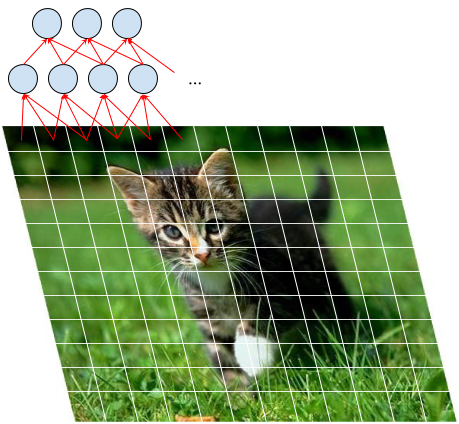
\includegraphics[natwidth=474,natheight=504,scale=0.6]{figures/cnnOnImage.png}
				\caption{L\textquotesingle image d\textquotesingle entr\'ee contient ici 166 composantes, donc la couche d\textquotesingle entr\'ee contiendra 166 neurones. On peut voir que la premi\`ere couche cach\'ee est bien un ensemble de pixel.}
				\label{fig:cnnChat}
			\end{figure}

			Pour les s\'eries temporelles, les CNN peuvent aussi s\textquotesingle appliquer. Par exemple, l\textquotesingle article de Zheng et coll. (\cite{zheng2014time}) utilise les CNN pour faire de la classification de s\'eries temporelles multivari\'ees, c\textquotesingle est \`a dire des s\'eries temporelles qui sont sur plusieurs dimensions.

	\subsection{Le manque de donn\'ee}
		Que faire lorsque l\textquotesingle on n\textquotesingle a pas assez de donn\'ees.

		\subsubsection{L\textquotesingle augmentation de donn\'ees}
			\medbreak

			\begin{itshape}{Pourquoi chercher \`a augmenter la base de donn\'es ?}\end{itshape}

			On a besoin de palier le manque de donn\'ee car les architectures de r\'eseau de neurones profond, comme les CNN, ont besoin de beaucoup de donn\'ees pour pouvoir \^etre entra\^in\'es efficacement. Les structures tels que MC-DCNN de Zheng et coll. (\cite{zheng2014time}) peuvent \^etre utilis\'e.
			De plus il y a peu, compar\'es aux images, de donn\'ees label\'ees sur les s\'eries temporelles. On aura donc besoin d\textquotesingle augmenter ces donn\'ees de diff\'erentes fa\c cons.
			Par analogie aux images, on regardera comment transformer une s\'erie temporelle. Dans les donn\'ees pour les images, on applique certaines transformations (\cite{krizhevsky2012imagenet,howard2013some}), tel que la translation, l\textquotesingle inversion, le changement de couleur, de contraste, de luminosit\'e, ... (figure~\ref{fig:dataAugmentationChat}). Ces transformations ne sont pas forc\'ement applicables aux s\'eries temporelles et on regardera donc comment faire.

			\medbreak

			\begin{itshape}{Comment y parvenir ?}\end{itshape}
			
			Pour les images, plusieurs techniques existent. Par exemple, Chatfield et coll. (\cite{chatfield2014return}) explique que pour r\'ealiser une augmentation de donn\'ees, ils perturbent une image avec des transformations qui n\textquotesingle invalide pas cette image, c\textquotesingle est \`a dire que si l\textquotesingle image d\textquotesingle origine montrait un chat, l\textquotesingle image transform\'ee doit toujours montrer un chat. Krizhevsky et coll. (\cite{krizhevsky2012imagenet}) explique que pour augmenter ses donn\'ees, il s\'epare tout d\textquotesingle abord ses donn\'ees en deux parties, l\textquotesingle une pour l\textquotesingle apprentissage, et l\textquotesingle autre pour les tests. Dans les donn\'ees pour l\textquotesingle apprentissage, ils r\'ealisent des sous-images en extractant des zones de 224x224 pixels de l\textquotesingle image d\textquotesingle origine et de sa r\'eflection horizontale, qui a une taille de 256x256. On obtient donc une multiplication de 2048 de la base de donn\'ees d\textquotesingle origine. Les donn\'ees de test prendront 5 sous-images et leur r\'eflection (donc 10 images) selon leurs pr\'edictions. Toujours dans l\textquotesingle id\'ee d\textquotesingle augmenter leurs donn\'ees d\textquotesingle apprentissage, ils effectuent une ACP pour pouvoir, non pas r\'eduire les dimensions, ajouter du bruit contr\^ol\'e sur les composants principaux. Krizhevsky et al. [5] arrivent donc \'a baisser le taux d\textquotesingle erreur de plus de 1\% ainsi. Dans le papier [6], Howard utilise le m\^eme proc\'ed\'e mais rajoute d\textquotesingle encore d\textquotesingle autres \'etapes. 

			\begin{figure}[!ht]
				\centering
				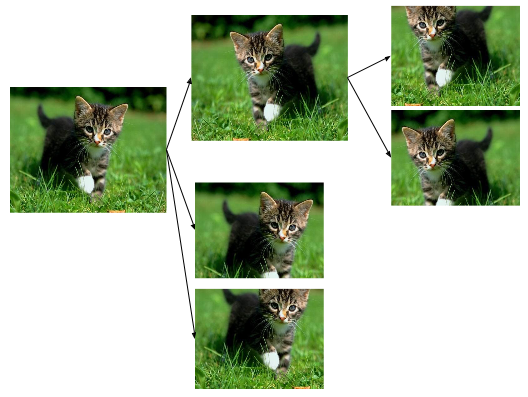
\includegraphics[scale=0.6,natwidth=528,natheight=397]{figures/dataAugmentationImage.png}
				\caption{Exemple d\textquotesingle augmentation de donn\'ee pour une image. Ici, on a obtenu six images \`a partie d\textquotesingle une seule. On a d\textquotesingle abord appliqu\'e une inversion d\textquotesingle image et puis on a rogn\'e les images obtenues de deux mani\`eres diff\'erentes. En r\'ealit\'e, beaucoup plus de transformations sont appliqu\'ees, permettant de multiplier la base de donn\'ees des images de beaucoup (1024 dans~\cite{howard2013some}).}
				\label{fig:dataAugmentationChat}
			\end{figure}

			Beaucoup de m\'ethode de data-augmentation le sont pour les images, la question \'etant de savoir si parmi ces m\'ethodes, on peut en r\'eutiliser ou non. Par exemple, on ne peut pas r\'ealiser une r\'eflection sur une s\'erie temporelle. Cependant, l\textquotesingle approche de Krizhevsky dans \cite{krizhevsky2012imagenet} pour les donn\'ees d\textquotesingle entra\^inement avec une ACP pourrait \^etre r\'ealisable sur des s\'eries temporelles. On pourrait peut-\^etre aussi rajouter du bruit contr\^ol\'e selon diff\'erents param\`etres comme dans \cite{krizhevsky2012imagenet} ou \cite{howard2013some}.

		\subsubsection{Dropout}
			Le dropout (vient de la contraction de deux mots anglais \textit{dropping out}) est une m\'ethode d\textquotesingle apprentissage qui permet d\textquotesingle obtenir de bons r\'esultats avec un nombre de donn\'ees r\'eduites. L\textquotesingle article de Srivastava et coll. (\cite{srivastava2014dropout}) introduite cette notion. Le principe est de d\'esactiver certains neurones par couches al\'eatoirement (figure~\ref{fig:dropout}).

			\begin{figure}[!ht]
				\centering
				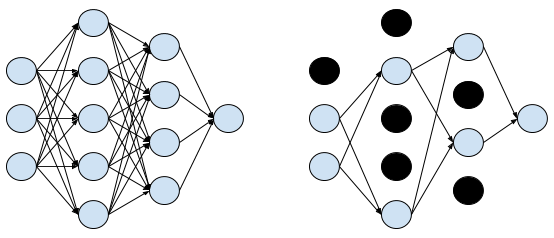
\includegraphics[scale=0.6,natwidth=554,natheight=238]{figures/dropout.png}
				\caption{Par exemple, le r\'eseau de neurone \`a droite est celui de gauche apr\`es que l\textquotesingle on est appliqu\'e le dropout. Comme on peut le voir, on r\'eduit de beaucoup de nombre de connexion entre les neurones.}
				\label{fig:dropout}
			\end{figure}

			On applique en faite une probabilit\'e \`a chaque couche. Par exemple, une probabilit\'e de 0.5 sur la couche $l$ d\textquotesingle un r\'eseau de neurone signifie que les neurones de cette couche ont chacun une probabilt\'e de 0.5 d\textquotesingle \^etre activ\'e. On note $p$ la probabilit\'e et on a donc la formule~(\ref{eq:zGlobal}) qui devient :

			\begin{equation}
				r_j^{(l)} ~~ Bernouilli(p)
				\label{eq:bernouilli}
			\end{equation}

			\begin{equation}
				\~a^{(l)} = r^{(l)} * a^{(l)}
				\label{eq:activationDropout}
			\end{equation}

			\begin{equation}
				z_i^{(l)} = \sum_{k=0}^{n^{(l-1)}} w_{ik}^{(l)} \~a_k^{(l-1)} \enskip \forall 1 < l \leq L
				\label{eq:zDropout}
			\end{equation}

			On comprend donc que la probabilit\'ee $p$ est une valeur qui influencer l\textquotesingle efficacit\'e du dropout. En effet, si $p$ est trop grand (proche de 1), on se rapproche trop d\textquotesingle un apprentissage classique, et ne pr\'esente donc que peu d\textquotesingle. Au contraire, si $p$ trop petit, le r\'eseau aura beaucoup de difficult\'e \`a apprendre car tr\`es peu de neurone. Srivastava et coll. (\cite{srivastava2014dropout}) nous informe que choisir $p = 0.5$ donne en g\'en\'eral de bons r\'esultats.


\bigbreak
\bigbreak
\section{Conclusion}
Pour conclure , il existe de nombreuses mani\`eres d\textquotesingle augmenter le volume des donn\'ees. Cependant, ces m\'ethodes d\'ependent du type de donn\'ees. Avant de commencer \`a classifier des s\'eries temporelles, il va donc falloir trouver comment augmenter ce volume. Nous pourrions, par exemple, utiliser l\textquotesingle agorithme ACP ou s\textquotesingle inspirer des m\'ethodes utilis\'es sur les images.
Pour la classification, les CNN semblent \^etre un bon choix \'etant donn\'ee les bons r\'esultats obtenus par Zheng et coll. (\cite{zheng2014time}). Pour cela, nous allons utiliser le framework Caffe (voir \cite{jia2014caffe}). Une fois mis en place, nous pourrions alors observer les r\'esultats.



\nocite{*}
\bibliographystyle{plain}
\bibliography{biblio}



\end{document}
%%% Local Variables:
%%% mode: latex
%%% TeX-master: t
%%% End:
